\chapter{Governing Equations}
\label{equation_chap}

The ARW dynamics solver integrates the compressible, nonhydrostatic
Euler equations.  The equations are cast in flux form using variables
that have conservation properties, following the philosophy of \citet{ooyama90}.
The equations are formulated using hydrostatic pressure as an independent variable
\citep{laprise92}. The vertical coordinate is terrain following, using a hybrid $\sigma-p$ formulation. In this chapter we define the vertical coordinate, present the moist flux-form equations in Cartesian
space, and augment the equations to include projections to the sphere.

\section{Vertical Coordinate and Flux-Form Variables}

%\begin{figure}
%\begin{center}
%  \includegraphics *[height=6cm,bb= 0 0 445.5 405.2]{../fig0.pdf}
%\end{center}
%  \caption{\label{figure:2} Terrain-following coordinate in {\wrf}}
%\end{figure}
%
%
%\begin{wrapfigure}{r}{8cm}
%mbox{
%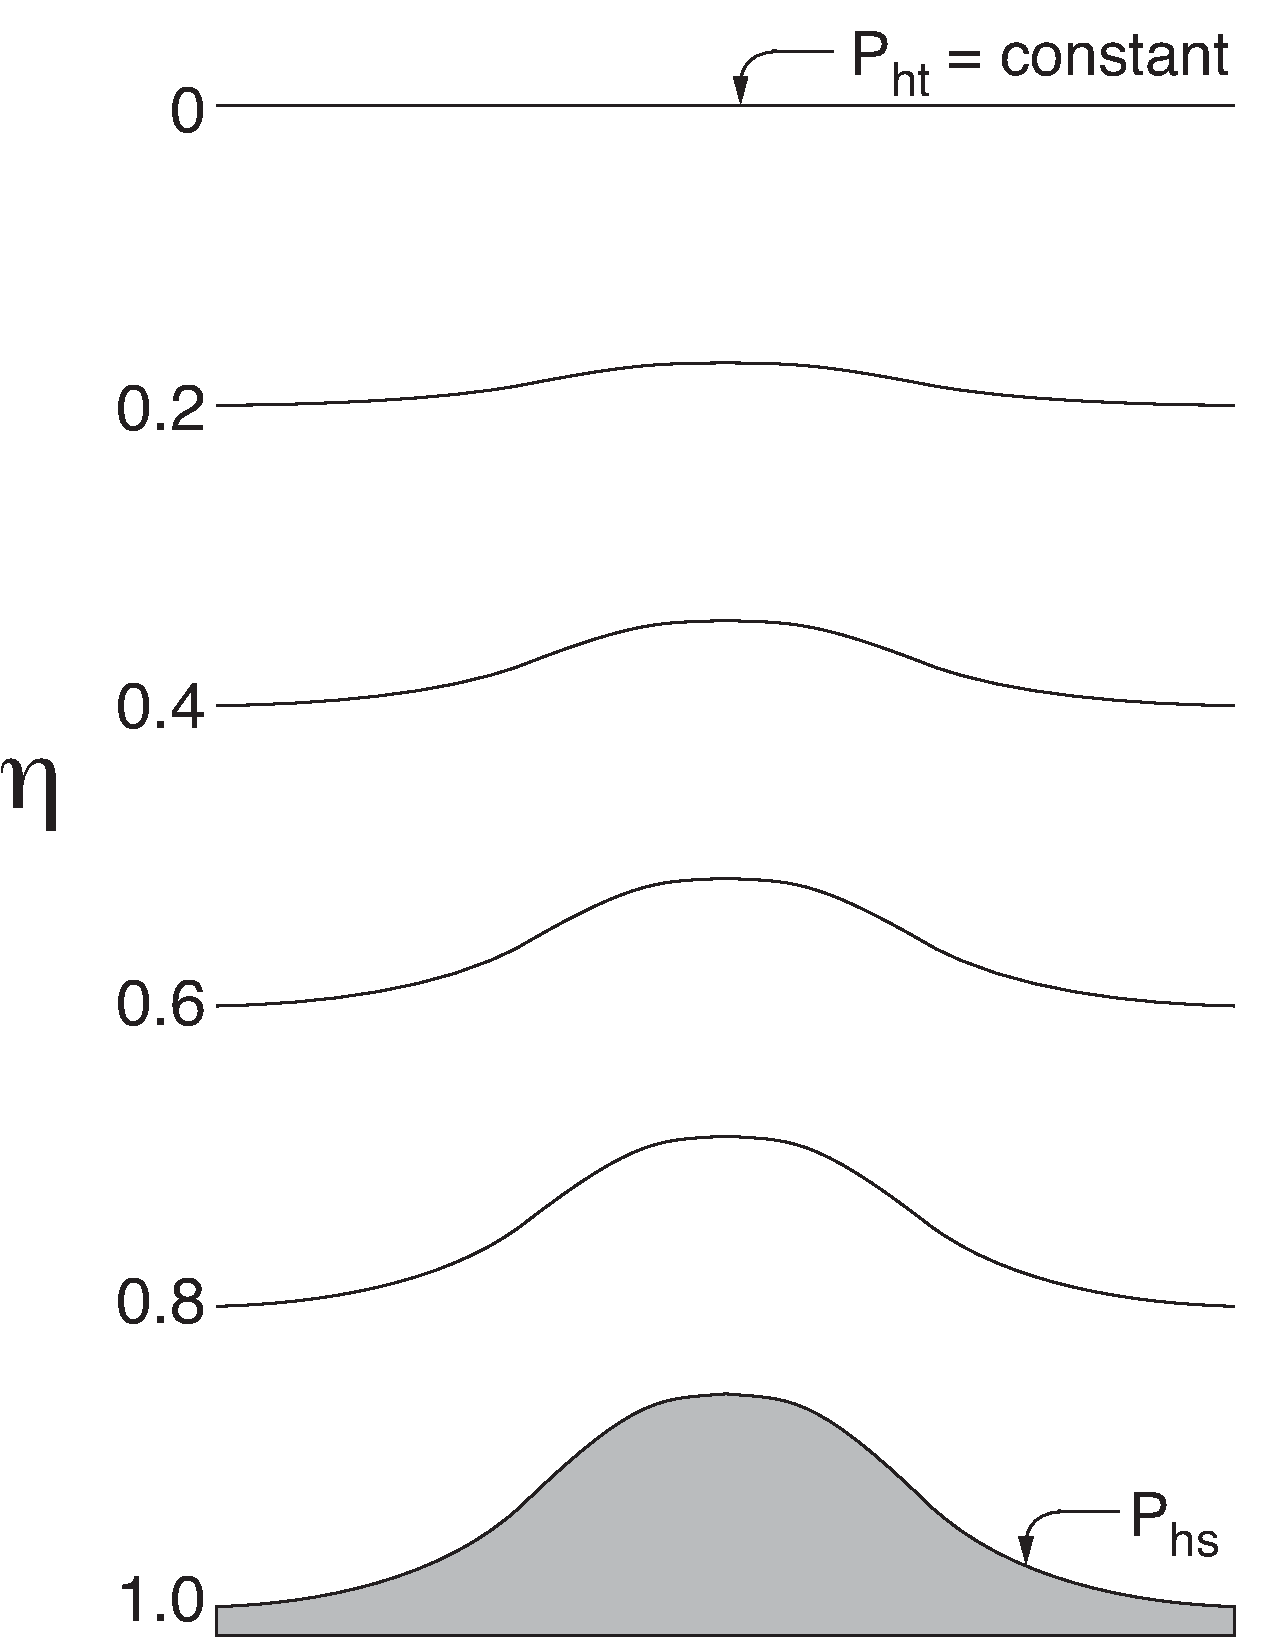
\epsfig{file=figures/vertical_coordinate.pdf,width=7cm,height=9.75cm}}
%\caption{\label{figure:v_coord}ARW $\eta$ coordinate.}
%\end{wrapfigure}
The ARW equations are formulated using a terrain-following
hydrostatic-pressure vertical coordinate denoted by $\eta$, which is also referred to a mass 
vertical coordinate. In previous versions of the ARW, $\eta$ was defined as
%
\begin{equation}
\eta = {p_d-p_{t}\over p_{s}-p_{t}},
\label{eta_def}
\end{equation}
where $p_d$ is the hydrostatic component of the pressure of dry air, and
$p_{s}$ and $p_{t}$ refer to values of $p_d$ along the surface and top
boundaries, respectively. The coordinate definition \eqref{eta_def},
proposed by \citet{laprise92} for use with the nonhydrostatic equations, 
is the traditional sigma coordinate used
in many hydrostatic atmospheric models.  $\eta$ varies from a value of 1
at the surface to 0 at the upper boundary of the model domain (Fig. \ref{figure:v_coord}a).

%
% Figure 2.1 something
%
\begin{figure}
 % \includegraphics *[width=6.5in,bb= 0 0 900 300]{figures/vertical_coordinate_new.pdf}
\centerline{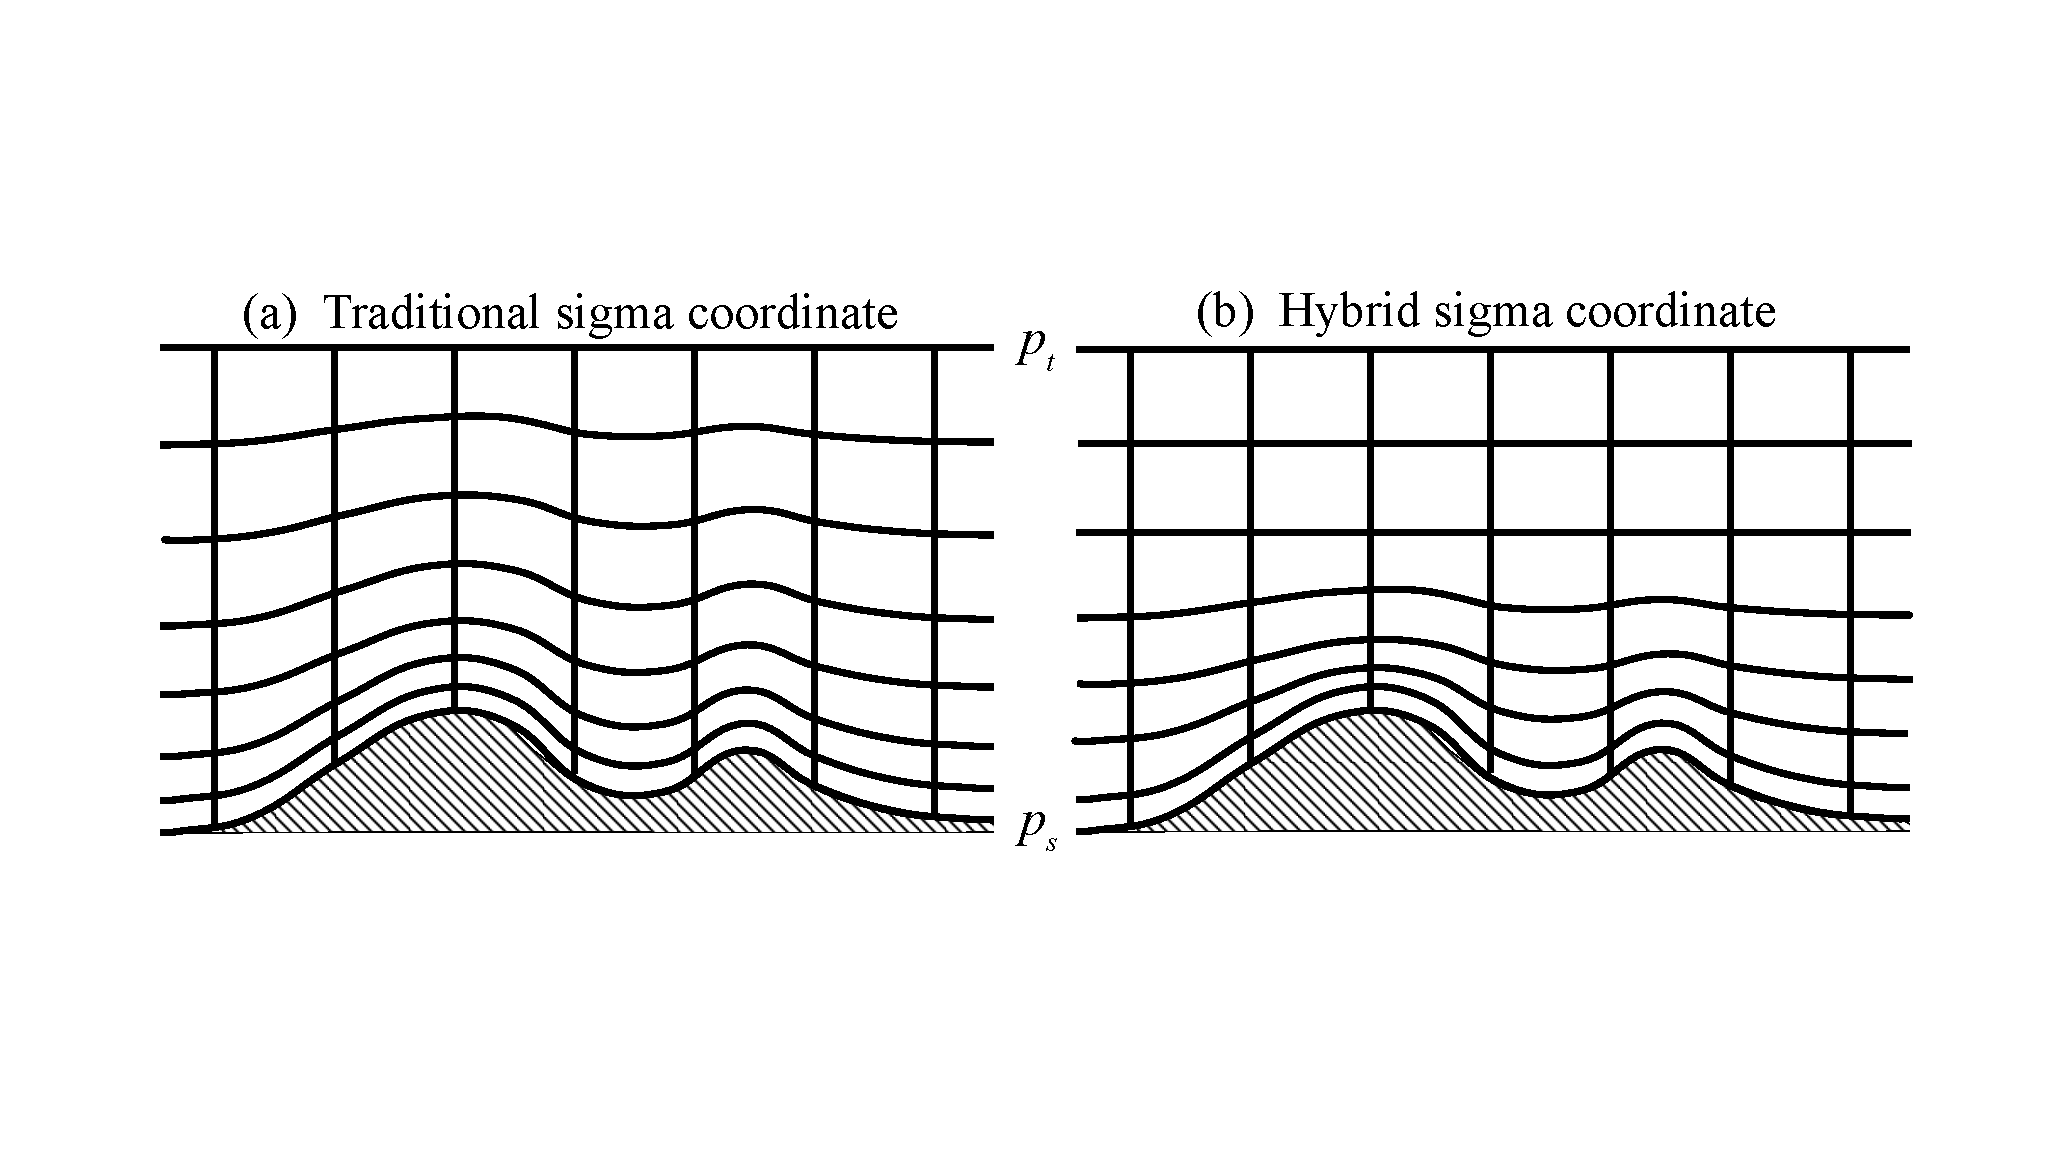
\includegraphics[width=38pc]{figures/vertical_coordinate_new.pdf}}
\caption{\label{figure:v_coord}ARW $\eta$ coordinate.}
\end{figure}

In the ARW Version, 4 the vertical coordinate has been generalized to allow the
influence of the terrain on the coordinate surfaces to be removed more rapidly
with increasing height above the surface, as illustrated in Fig. \ref{figure:v_coord}b. For this modified  vertical coordinate, we employ a hybrid sigma-pressure vertical coordinate as described by \citet{park13}, which is similar to that used in the National Center for Atmospheric Research (NCAR) Community Atmospheric Model (CAM),as described in the NCAR CAM3.0 Technical Note:
%
\begin{equation}
p_d = B(\eta)(p_{s}-p_t) + [\eta-B(\eta)](p_0-{p_t})+p_t,          
\label{hyb_def}
 \end{equation}
%
where $p_0$ is a reference sea-level pressure. (This coordinate representation differs somewhat from CAM in that it is based on dry pressure instead of full pressure and is normalized using $p_t$ such that $\eta=0$ at $p_d = p_t$.) Here, $B(\eta)$ defines the relative weighting between the terrain-following sigma coordinate and a pure pressure coordinate, such that $\eta$ corresponds to the sigma coordinate \eqref{eta_def} for $B(\eta) = \eta$ and reverts to a hydrostatic pressure coordinate for $B(\eta) = 0$. To smoothly transition from a sigma coordinate near the surface to a pressure coordinate at upper levels, $B(\eta)$ is defined by a third order polynomial
%
\begin{equation}
B(\eta) = c_1+c_2\eta+c_3\eta^2+c_4\eta^3         
\label{B_def}
 \end{equation}
%
(where the subscript $\eta$ denotes differentiation) subject to the boundary conditions
%
\begin{equation}
B(1)=1,\quad B_\eta(1)=1, \quad B(\eta_c)=0, \quad B_\eta(\eta_c)=0,         
\label{B_bc}
 \end{equation}
%
such that
%
\begin{equation}
c_1={2\eta_c^2\over(1-\eta_c)^3},  \quad      
c_2={-\eta_c(4+\eta_c+\eta_c^2)\over(1-\eta_c)^3},  \quad      
c_3={2(1+\eta_c+\eta_c^2)\over(1-\eta_c)^3},  \quad      
c_4={-(1+\eta_c)\over\ \ \ (1-\eta_c)^3},    
\label{B_cof}
 \end{equation}
where $\eta_c$ is a specified value of $\eta$ at which it becomes a pure pressure coordinate.%
% Figure 2.2 something
%
\begin{figure}
 % \includegraphics *[width=6.5in,bb= 0 0 900 300]{figures/vertical_coordinate_new.pdf}
\centerline{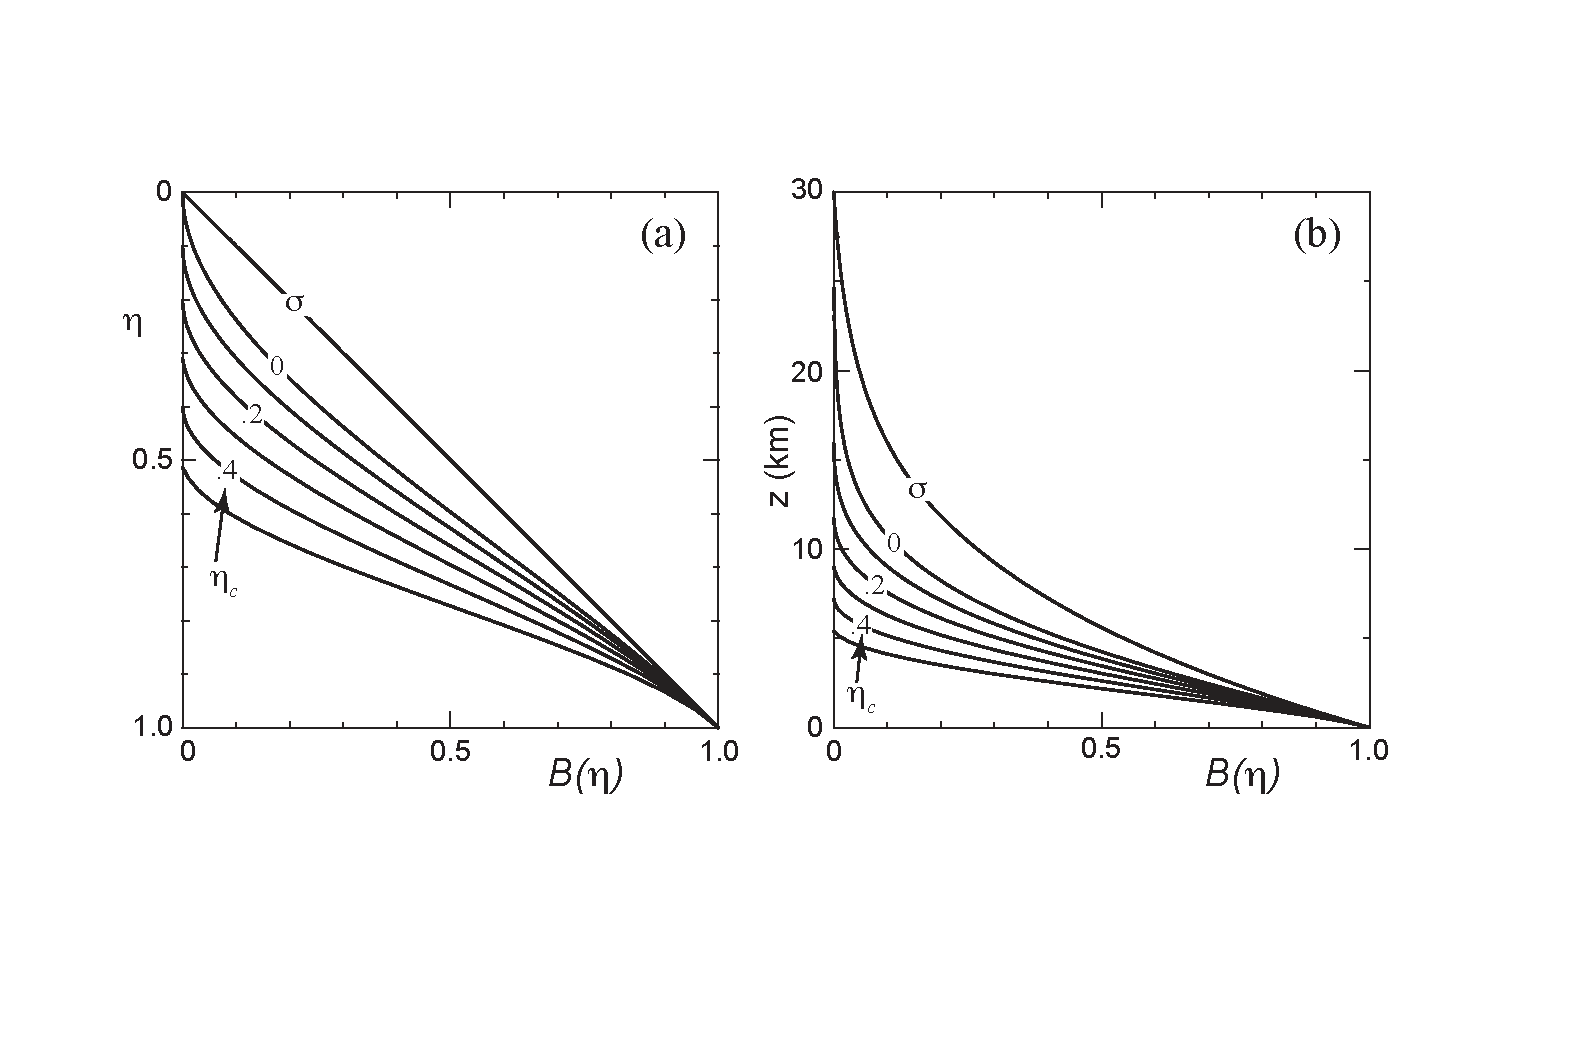
\includegraphics[width=38pc]{figures/B_profile.pdf}}
\caption{\label{figure:B_profile}B($\eta$) profiles for sigma ($\sigma$) coordinate and for hybrid coordinate for $\eta_c=0.,0.1,\,0.2,\,0.3,\,0.4,\,$ and $0.5$ displayed (a) as a function of $\eta$, and (b) as a function of height for a standard atmosphere in a domain with a 30 km upper boundary.}
\end{figure}

Figure \ref{figure:B_profile} displays the $B(\eta)$ profiles for the traditional sigma coordinate and for the hybrid coordinate for several values of the parameter $\eta_c$. Plotted as a function of $\eta$ (Fig. \ref{figure:B_profile}a), these profiles depict the form of the polynomial defined in \eqref{B_def}. However, plotting $B(\eta)$ as a function of height  (Fig. \ref{figure:B_profile}b) provides a better physical sense of the transition toward a pressure coordinate with increasing height. For example, with a model domain having a depth of 30 km, for $\eta_c=0.2$ the vertical coordinate becomes a pure pressure coordinate at an altitude of about 12 km.

%
The vertical coordinate metric is defined as 
%
\begin{equation}
\mu_d= {\partial p_d\over\partial\eta} = B_\eta(\eta)(p_s-p_t) +[1-B_\eta(\eta)](p_0-p_t). \label{mu_def}
\end{equation}
%
Since $\mu_d \Delta\eta=\Delta p_d=-g\rho_d \Delta z$ is proportional to the mass per unit area within a
grid cell, the appropriate flux forms for the prognostic  variables are defined as
%
\begin{equation}
 \hbox{\bf V} = \mu_d \hbox{\bf  v} =(U,V,W), ~~~~ \Omega = \mu_d\omega, ~~~~ 
     \Theta_m = \mu_d \theta_m, ~~~~ Q_m = \mu_d q_m.                                      
\end{equation}
%
\noindent
Here, ${\hbox{\bf v}} = (u,v,w)$ are the covariant velocities in the
horizontal and vertical directions, while 
$\omega = \dot\eta$ is the contravariant `vertical' velocity.  $\theta_m = \theta (1 + (R_v/R_d) q_v) 
\approx \theta (1 + 1.61 q_v)$ is the moist potential temperature and $Q_m = \mu_d q_m$, where $q_m = q_v, q_c,
q_r ...$ represents the mixing ratios of moisture variables (water vapor, cloud water, rain water, ...).  Although the geopotential $\phi=gz$ is also a prognostic variable in the governing equations of the ARW, it is not written in flux-form as $\mu_d\phi$ is not a conserved quantity. 
 
\section{Flux-Form Euler Equations}

Using the variables defined above, the flux-form Euler equations can be
written as
%
\begin{align}
\partial_t U + (\nabla \cdot {\bf V}  u)
+ \mu_d \alpha \partial_x p 
+ (\alpha/\alpha_d) \partial_\eta p \partial_x \phi & = F_U \label{U_eq}\\
%
\partial_t V + (\nabla \cdot {\bf V} v ) 
+ \mu_d \alpha \partial_y p
+ (\alpha/\alpha_d) \partial_\eta p \partial_y \phi & = F_V \label{V_eq}\\
%
\partial_t W + (\nabla \cdot {\bf V} w )  
- g [ (\alpha/\alpha_d) \partial_\eta p - \mu_d ] & = F_W \label{W_eq}\\
%
\partial_t \Theta_m + (\nabla \cdot {\bf V} \theta_m )  & = F_{\Theta_m} \label{T_eq}\\
%
\partial_t \mu_d + (\nabla \cdot {\bf V} ) & = 0 \label{mu_eq}\\
%
\partial_t \phi + \mu_d^{-1} [({\bf V} \cdot \nabla \phi ) - gW ] & = 0 \label{phi_eq}\\
%
\partial_t Q_m + (\nabla \cdot {\bf V} q_m ) & = F_{Q_m} \label{Q_eq}
%
\end{align}
\noindent
with the diagnostic equation for dry hydrostatic pressure
%
\begin{equation}
\partial_\eta \phi  = - \alpha_d \mu_d \label{pd_eq}
\end{equation}
%
\noindent
and the diagnostic relation for the 
full pressure (dry air plus water vapor)
%
\begin{equation}
p = p_0 {\left({R_d \theta_m \over p_0 \alpha_d}\right)}^{\gamma}.
\label{ideal_gas_law}
\end{equation}
%
\noindent
In these equations, $\alpha_d$ is the inverse density of the dry air
$(1/\rho_d)$ and $\alpha$ is the inverse density taking into account the
full parcel density 
$\alpha = \alpha_d ( 1 + q_v + q_c + q_r + q_i + ...)^{-1}$. 

In (\ref{U_eq}) -- (\ref{Q_eq}), the subscripts 
$x$, $y$ and $\eta$ denote
differentiation, 
%
\begin{equation}
\nabla \cdot {\bf V } a = \partial_x (Ua) + 
                           \partial_y (Va) + 
                           \partial_\eta (\Omega a),
\notag
\end{equation}
%
\noindent
and
%
\begin{equation}
{\bf V} \cdot \nabla a = U \partial_x a + 
                           V \partial_y a + 
                           \Omega \partial_\eta a,
\notag
\end{equation}
%
\noindent
where $a$ represents a generic variable.  
$\gamma=c_p/c_v = 1.4$ is the ratio of
the heat capacities for dry air, $R_d$ is the gas constant for dry
air, and $p_0$ is a reference surface pressure (typically $10^5$ Pascals).
The right-hand-side (RHS) terms $F_U$, $F_V$, $F_W$, and
$F_{\Theta_m}$ represent forcing terms arising from model physics,
turbulent mixing, spherical projections, and the earth's rotation.

In specifying the prognostic set of equations, a prognostic pressure equation could be used in
place of \eqref{phi_eq} \citep[see][]{laprise92}. However, pressure is
not a conserved variable and with pressure as a prognostic variable we could not use the conservation equation \eqref{T_eq} for $\Theta_m$  because
they are linearly dependent.  
Additionally, prognostic pressure
equations have the disadvantage of possessing a mass divergence term
multiplied by a large coefficient (proportional to the sound speed)
which makes spatial and temporal discretization problematic.
It should be noted that the relation for the dry hydrostatic pressure
\eqref{pd_eq} does not impose a hydrostatic constraint on
the solution, rather it is a diagnostic relation that formally is part
of the coordinate definition.  In the hydrostatic counterpart to the
nonhydrostatic equations, the full hydrostatic equation $\partial_\eta p=\mu_d\alpha_d/\alpha$ replaces the
vertical momentum equation \eqref{W_eq} and enforces a hydrostatic 
constraint on the solution.

In previous versions of the ARW the prognostic thermodynamic equation was expressed in terms of $\Theta$ instead of $\Theta_m$ in \eqref{T_eq}. That representation is consistent with the expectation that variations in $q_v$ have little impact during the small acoustic time steps in the split-explicit numerics described in the next chapter, which has proven to be a robust approximation over a wide spectrum of applications. However, in a recent study, \citet{xiao15} found that in high-resolution LES with sharp vertical variations in water vapor, WRF simulations exhibited a strong sensitivity to the time step used to accommodate the acoustic modes. Recasting the prognostic thermodynamic equation in terms of $\Theta_m$ allowed consistent treatment of moisture in the calculation of pressure during the acoustic time steps, and spurious motions and time-step sensitivity were eliminated. Use of $\Theta_m$ as the prognostic thermodynamic variable is also consistent with formulation used in the Model for Prediction Across Scales (MPAS), which utilizes similar split-explicit numerics \citep{skamarock12}.


\section{Map Projections, Coriolis and Curvature Terms}
\label{spherical_projections}

The ARW solver currently supports four projections to the sphere--- the
Lambert conformal, polar stereographic, Mercator, and latitude-longitude
projections.  These projections are described in
\citet{haltiner_and_williams}.  The transformation is isotropic for
three of these projections -- the Lambert conformal, polar stereographic,
and Mercator grids.  An isotropic transformation requires $(\Delta
x/\Delta y)|_{earth} = \hbox{constant}$ everywhere on the grid.  Only
isotropic transformations were supported in the previous ARW releases.
Starting with the ARWV3 release, we now support anisotropic
projections, in this case the latitude-longitude grid, and with it the
full latitude-longitude global model.  The ARW implements the
projections using map factors, and the generalization to anisotropic
transformations introduced in ARW V3 requires that there be map factors
for both the $x$ and $y$ components of the transformation from
computational to physical space in order to accommodate the anisotropy.

In the ARW's computational space, $\Delta x$ and $\Delta y$ are
constants.  Orthogonal projections to the sphere require that
the physical distances between grid points in the projection vary with
position on the grid.  To transform the governing equations,
map scale factors $m_x$ and $m_y$ are defined as the ratio of the distance 
in computational space to the corresponding distance on the earth's surface:

\begin{equation}
(m_x,m_y) = {(\Delta x, \Delta y) \over \hbox{distance on the earth}}.
\label{map_scale}
\end{equation}
%
\noindent
The ARW solver includes the map-scale factors in the governing equations
by redefining the momentum variables as
%
\begin{equation}
U = {\mu}_d u/m_y,~~~V = {\mu}_d v/m_x, ~~~W = \mu_d w / m_y, 
~~~\Omega = \mu_d \omega /m_y.
\notag
\end{equation}
%
\noindent
Using these redefined momentum variables, 
the governing prognostic equations \eqref{U_eq}-\eqref{Q_eq} including map factors 
can be written as
%
\begin{align}
\partial_t U + m_x[\partial_x(Uu) + \partial_y(Vu)] \hphantom{\quad\quad\quad\quad\quad\quad\quad\quad\quad\quad\quad\quad\quad\quad\quad\quad\quad\quad\quad\quad}
\notag \\ 
+ \hphantom{(m_y/m_x)} 
\partial_\eta (\Omega u)
+ (m_x/m_y)[\mu_d \alpha \partial_x p
+ (\alpha/\alpha_d) \partial_\eta p \partial_x \phi] & = F_U
\label{u-mom-full}
\\
%
\partial_t V + m_y[\partial_x (Uv) + \partial_y (Vv)] \hphantom{\quad\quad\quad\quad\quad\quad\quad\quad\quad\quad\quad\quad\quad\quad\quad\quad\quad\quad\quad\quad}
\notag \\ + (m_y/m_x)\partial_\eta (\Omega v)
+ (m_y/m_x)[\mu_d \alpha \partial_y p
+ (\alpha/\alpha_d) \partial_\eta p \partial_y \phi] & = F_V
\label{v-mom-full}
\\
%
\partial_t W + m_x [\partial_x (Uw) + \partial_y (Vw)] + \partial_\eta (\Omega w)
- m_y^{-1} g [ (\alpha/\alpha_d) \partial_\eta p - \mu_d ] & = F_W 
\label{w-mom-full}
\\
%
\partial_t \Theta_m + 
m_x m_y[\partial_x (U\theta_m) + \partial_y (V\theta_m)] + m_y \partial_\eta (\Omega \theta_m)
& = F_{\Theta_m} 
\label{tm_full} \\
%
\partial_t \mu_d + m_x m_y[U_x + V_y] + m_y \partial_\eta (\Omega)
& = 0 
\label{mass-cons-full}
\\
%
%% \partial_t \phi + \mu_d^{-1} [m_x m_y (U\phi_x + V\phi_y) + m_y
%% \Omega\phi_\eta - m_y gW ] & = 0
\partial_t \phi + \mu_d^{-1} [m_x m_y (U\partial_x\phi + V\partial_y\phi) + m_y
\Omega\partial_\eta\phi - m_y gW ] & = 0
\label{geo-full}
\\
%
\partial_t Q_m + 
m_x m_y \partial_x (U q_m) + \partial_y (V q_m)] + m _y\partial_\eta (\Omega q_m)
& = F_{Q_m},
\label{qm_full}%
\end{align}
\noindent
which are solved together with the diagnostic equations \eqref{pd_eq} and \eqref{ideal_gas_law}.
%
%\begin{equation}
%\partial_\eta \phi  = - \alpha_d \mu_d,
%\label{hydro-full}
%\end{equation}
%
\noindent
%
%\begin{equation}
%p = p_0 (R_d \theta_m / p_0 \alpha_d)^{\gamma}.
%\label{moist-state-equation}
%\end{equation}
%

The right-hand-side terms of the momentum equations
\eqref{u-mom-full} -- \eqref{w-mom-full} contain the Coriolis and 
curvature terms along with mixing terms and 
physical forcings.  Including the map-scale factors \eqref{map_scale}, the Coriolis and
curvature terms are cast in the following form:

\begin{align}
F_{U_{cor}} & =  + {m_x\over m_y}
\ \ \Bigl(f + u {m_y\over m_x}{\partial m_x \over
\partial y} - v {\partial m_y \over \partial x}\Bigr) V
- \Bigl( {u \over r_e}  + e \cos \alpha_r \Bigr)W \label{u-mom-rhs} 
\\
%
F_{V_{cor}} & = - {m_y\over m_x}\biggl[ \Bigl(f + u {m_y\over m_x}{\partial m_x \over
\partial y} - v {\partial m_y \over \partial x}\Bigr) U
+ \Bigl( {v \over r_e} -e \sin \alpha_r \Bigr)W \biggr] \label{v-mom-rhs} 
\\
%
F_{W_{cor}} & = + e \Bigl(U \cos \alpha_r - {m_x\over m_y}V \sin \alpha_r\Bigr) 
+ {1\over r_e}\biggl(uU +{m_x\over m_y}vV \biggr), \label{w-mom-rhs}
\end{align}
\noindent
where $\alpha_r$ is the local rotation angle between the $y$-axis and the
meridians, $\psi$ is the latitude, $f = 2 \Omega_e \sin \psi $, $e = 2
\Omega_e \cos \psi$, $\Omega_e$ is the angular rotation rate of the earth,
and $r_e$ is the radius of the earth.  In this
formulation we have approximated the radial distance from the center of
the earth as the mean earth radius $r_e$, and we have not taken into account
the change in horizontal grid distance as a function of the radius.
The terms containing the map-scale factors represent the horizontal curvature terms, those
containing $r_e$ relate to vertical (earth-surface) curvature, and those
with $e$ and $f$ are the Coriolis force.


 For the isotropic projections 
(Lambert conformal, polar stereographic, and Mercator), the map-scale factors are the same in both horizontal directions, such that $m_x=m_y=m$,
where $m$ typically only varies with latitude. 
For the anisotropic latitude-longitude grid, $m_x=\sec\psi$ and $m_y=1$, so that $\partial m_x/\partial y  = (1/r_e) \sec \psi \tan \psi$ and $\partial m_y/\partial x  = 0$, 
given that $\partial / \partial y = (1/r_e)\partial/\partial \psi$.
For idealized cases on a Cartesian grid, the map-scale factors $m_x = m_y = 1$, 
$f$ is specified, and $e$ and $r_e^{-1}$ should be zero to remove the curvature terms.

\section{Perturbation Form of the Governing Equations}

Before constructing the discrete solver, it is advantageous to recast
the governing equations using perturbation variables to reduce
truncation errors in the horizontal pressure gradient calculations in
the discrete solver and machine rounding errors in
the vertical pressure gradient and buoyancy calculations.  
For this purpose, new
variables are defined as perturbations from a hydrostatically-balanced 
reference state, and we define reference state
variables (denoted by overbars) that are a function of height only and
that satisfy the governing equations for an atmosphere at rest.  That is,
the reference state is in hydrostatic balance and is strictly only a
function of $\bar z$.  In this manner, $p=\bar p(\bar z)+p'$, $\phi=\bar
\phi(\bar z)
+\phi'$, $\alpha=\bar \alpha_d(\bar z) +\alpha_d'$, and $\mu_d = \bar\mu_d(x,y) +
\mu_d'$. Because the $\eta$ coordinate surfaces are generally not
horizontal, the reference profiles $\bar p$, $\bar\phi$, and
$\bar\alpha$ are functions of $(x,y,\eta)$. 
The hydrostatically balanced portion of the pressure gradients in the
reference sounding can be removed without approximation to the equations
using these perturbation variables.
The momentum equations 
\eqref{u-mom-full} -- \eqref{w-mom-full} are written as
%
\begin{align}
\partial_t U + m_x\left[\partial_x(Uu) + \partial_y(Vu)\right] + \partial_\eta (\Omega u) ~~~~~~~~ ~~~~~~~~ ~~~~~~~~ ~~~~~~~~ ~~~~~~~ ~~~~~~~ ~~ \notag &
\hphantom{(m_y/m_x)}
\\
+(m_x/m_y) (\alpha/\alpha_d) \left[ \mu_d (\partial_x \phi' + \alpha_d \partial_x p' + \alpha'_d \partial_x \overline{p}) +
\partial_x \phi (\partial_\eta p' - \mu'_d)\right]  = F_U
%%+ ({\mu}_d \alpha \partial_x p' 
%%+ {\mu}_d \alpha' \partial_x \bar{p}) ~~~~~~~~ \notag &
%%\\
%%+ (\alpha/\alpha_d) ( {\mu}_d \partial_x \phi' 
%%+  \partial_\eta p' \partial_x \phi 
%%- {\mu}_d' \partial_x \phi )
%%                                                       &= F_U  
\label{u-mom-pert}
\\
%
\partial_t V + m_y[\partial_x (Uv) + \partial_y (Vv)] + (m_y/m_x) \partial_\eta (\Omega v) ~~~~~~~~ ~~~~~~~~ ~~~~~~~~ ~~~~~~~~ ~~~~~~ \notag &
\\
+(m_y/m_x) (\alpha/\alpha_d) \left[ \mu_d (\partial_y \phi' + \alpha_d \partial_y p' + \alpha'_d \partial_y \overline{p}) +
\partial_y \phi (\partial_\eta p' - \mu'_d)\right]  = F_V
\\
%%+ ({\mu}_d \alpha \partial_y p' 
%%+ {\mu}_d \alpha' \partial_y \bar{p}) ~~~~~~~~ \notag &
%%\\
%%+ (\alpha/\alpha_d) ( {\mu}_d \partial_y \phi' 
%%+ \partial_\eta p' \partial_y \phi 
%%- {\mu}_d' \partial_y \phi )
%%                                                      &= F_V   \\ 
%
\partial_t W  + m_x [\partial_x (Uw) + \partial_y (Vw)] + \partial_\eta
(\Omega w)  ~~~~~~~~ ~~~~~~~~ ~~~~~~~~ ~~~~~~~~ ~~~ \notag & 
\\
- m_y^{-1} g (\alpha/\alpha_d) [\partial_\eta p' 
- {\bar{\mu}}_d (q_v + q_c +q_r)]
+ m_y^{-1} {\mu}_d'g
&= F_W,
\label{w-mom-pert}
\end{align}
%
and the mass conservation equation \eqref{mass-cons-full}
and geopotential equation \eqref{geo-full} become
%
\begin{align}
\partial_t  \mu_d' + m_x m_y[\partial_x U + \partial_y V] + m_y
\partial_\eta \Omega
& = 0 \\
%
\partial_t \phi' 
+ \mu_d^{-1}
%% [m_x m_y (U\phi_x + V\phi_y) + m_y
%% \Omega\phi_\eta -m_y gW ] = 0.
[m_x m_y (U\partial_x\phi + V\partial_y\phi) + m_y
\Omega\partial_\eta\phi -m_y gW ] = 0,
\label{phi_pert}
%
\end{align}
%
\noindent
and the diagnostic equation for dry hydrostatic pressure \eqref{pd_eq} becomes
%
\begin{equation}
\partial_\eta \phi' =-\bar\mu_d \alpha'_d-\alpha_d\mu'_d.
\label{hydro-pert}
\end{equation}
%
Additionally, an option is available to use the hypsometric equation for the dry hydrostatic pressure in place of (\ref{hydro-pert}):
\begin{equation}
%{1 \over p}{\partial \phi \over \partial (\ln p)} = - \bar \alpha - \alpha'
{\partial \phi / \partial (\ln p_d)} = - p_d(\bar \alpha_d + \alpha'_d).
\label{hypsometric_eqn}
\end{equation}
%
This form of the hydrostatic relation can produce a more accurate discretization compared with (\ref{hydro-pert}) when the variation with $\eta$ of temperature 
$(p_d \alpha_d)$ is more linear than that of density $(\alpha_d^{-1})$.
The conservation equations for the potential temperature \eqref{tm_full} and 
the scalar moisture equations \eqref{qm_full} remain unchanged.

Equations \eqref{u-mom-pert} -- \eqref{hydro-pert},
together with the equation of state \eqref{ideal_gas_law},
represent the equations solved in the ARW.
The RHS terms in these equations include the
Coriolis terms \eqref{u-mom-rhs} -- \eqref{w-mom-rhs},
mixing terms (described in Chapter \ref{filter_chap}), and
parameterized physics (described in Chapter \ref{physics_chap}).  
Also note that the equation of state \eqref{ideal_gas_law} cannot be
written in perturbation form because of the exponent in the expression.
For small perturbation simulations, accuracy for perturbation variables
can be maintained by linearizing \eqref{ideal_gas_law} for the
perturbation variables.
%


